\documentclass[border=6pt]{standalone}
\usepackage{lmodern}
\usepackage[T1]{fontenc}
\usepackage{amsmath}
\usepackage{bm}
\usepackage{xcolor}
\usepackage{tikz}
\usetikzlibrary{arrows.meta,positioning}
\definecolor{cgray}{HTML}{6E6C66}
\definecolor{cblue}{HTML}{2F7DC8}
\definecolor{camber}{HTML}{E0891E}
\definecolor{cgreen}{HTML}{4E8E2A}
\definecolor{cred}{HTML}{C0392B}
\definecolor{cink}{HTML}{2B2B2B}
\tikzset{
  >={Stealth[length=2.2mm]},
  crv/.style={line width=1.0pt,cink,smooth,samples=120},
}
\newcommand{\gauss}[1]{2.0*exp(0-(#1*#1)/1.4)}
\begin{document}
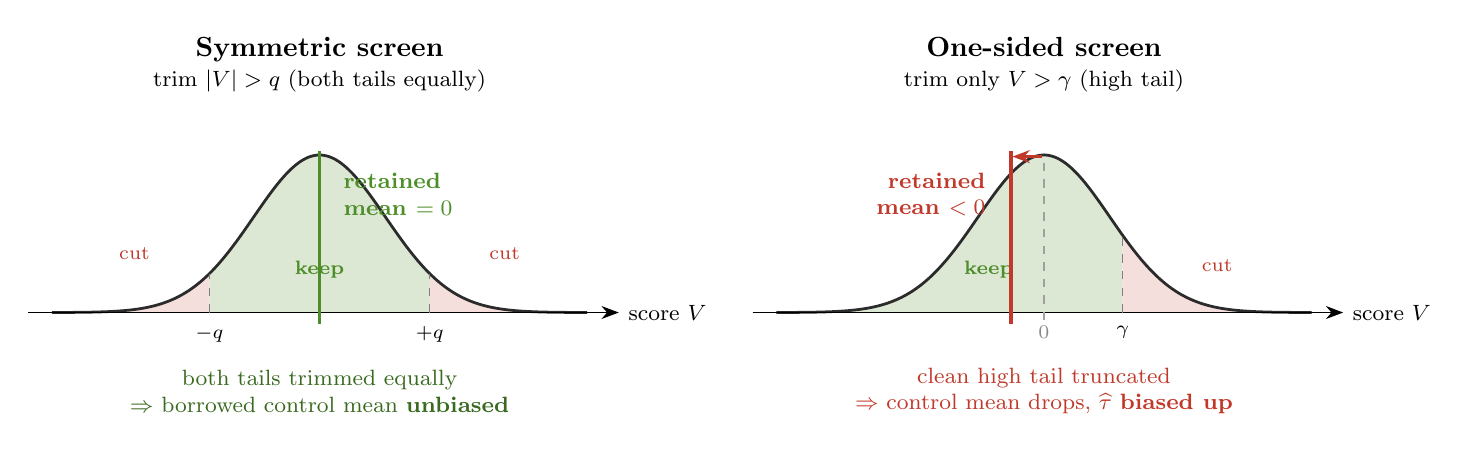
\begin{tikzpicture}[font=\small]

% ================= PANEL A : symmetric =================
\begin{scope}
  \node[font=\bfseries,align=center] at (0,3.15) {Symmetric screen \\[-1pt] \footnotesize\mdseries trim $|V|>q$ (both tails equally)};
  % kept centre (green)
  \fill[cgreen!20] (-1.4,0) -- plot[domain=-1.4:1.4,samples=60] (\x,{\gauss{\x}}) -- (1.4,0) -- cycle;
  % cut tails (red)
  \fill[cred!16] (1.4,0) -- plot[domain=1.4:3.4,samples=40] (\x,{\gauss{\x}}) -- (3.4,0) -- cycle;
  \fill[cred!16] (-3.4,0) -- plot[domain=-3.4:-1.4,samples=40] (\x,{\gauss{\x}}) -- (-1.4,0) -- cycle;
  \draw[crv] plot[domain=-3.4:3.4] (\x,{\gauss{\x}});
  \draw[->] (-3.7,0) -- (3.8,0) node[right,font=\footnotesize]{score $V$};
  \draw[dashed,cink!60] (1.4,0) -- (1.4,{\gauss{1.4}}); \draw[dashed,cink!60] (-1.4,0) -- (-1.4,{\gauss{1.4}});
  \node[cred,font=\scriptsize] at (2.35,0.75) {cut}; \node[cred,font=\scriptsize] at (-2.35,0.75) {cut};
  \node[cgreen,font=\scriptsize\bfseries] at (0,0.55) {keep};
  \node[below,font=\scriptsize] at (1.4,-0.05){$+q$}; \node[below,font=\scriptsize] at (-1.4,-0.05){$-q$};
  % retained mean at 0
  \draw[cgreen,line width=1.3pt] (0,-0.15) -- (0,2.05);
  \node[cgreen,font=\footnotesize\bfseries,align=left,anchor=west] at (0.18,1.5) {retained\\ mean $=0$};
  \node[align=center,font=\footnotesize,text=cgreen!75!black] at (0,-1.0) {both tails trimmed equally\\ $\Rightarrow$ borrowed control mean \textbf{unbiased}};
\end{scope}

% ================= PANEL B : one-sided =================
\begin{scope}[xshift=9.2cm]
  \node[font=\bfseries,align=center] at (0,3.15) {One-sided screen \\[-1pt] \footnotesize\mdseries trim only $V>\gamma$ (high tail)};
  \def\gam{1.0}
  % kept region (green) from -3.4 to gamma
  \fill[cgreen!20] (-3.4,0) -- plot[domain=-3.4:\gam,samples=80] (\x,{\gauss{\x}}) -- (\gam,0) -- cycle;
  % cut high tail (red)
  \fill[cred!16] (\gam,0) -- plot[domain=\gam:3.4,samples=50] (\x,{\gauss{\x}}) -- (3.4,0) -- cycle;
  \draw[crv] plot[domain=-3.4:3.4] (\x,{\gauss{\x}});
  \draw[->] (-3.7,0) -- (3.8,0) node[right,font=\footnotesize]{score $V$};
  \draw[dashed,cink!60] (\gam,0) -- (\gam,{\gauss{\gam}});
  \node[cred,font=\scriptsize] at (2.2,0.6) {cut}; \node[cgreen,font=\scriptsize\bfseries] at (-0.7,0.55) {keep};
  \node[below,font=\scriptsize] at (\gam,-0.05){$\gamma$};
  % original mean 0 (faint) and shifted retained mean
  \draw[cink!45,dashed,line width=0.9pt] (0,-0.1) -- (0,2.02);
  \node[cink!55,font=\scriptsize,below] at (0,-0.05) {$0$};
  \draw[cred,line width=1.3pt] (-0.42,-0.15) -- (-0.42,2.05);
  \node[cred,font=\footnotesize\bfseries,align=right,anchor=east] at (-0.62,1.5) {retained\\ mean $<0$};
  \draw[->,cred,line width=0.9pt] (-0.02,1.98) -- (-0.4,1.98);
  \node[align=center,font=\footnotesize,text=cred] at (0,-1.0) {clean high tail truncated\\ $\Rightarrow$ control mean drops, $\widehat\tau$ \textbf{biased up}};
\end{scope}

\end{tikzpicture}
\end{document}
